\subsubsection{Triaxial compression strength tests (TC) for salt - methodology and equipment}
\index{triaxial compression test (TC)}

Triaxial compression tests (TC) are executed on cylindrical core samples with dimensions of e.g. 200*100 mm (generally a 2:1 ratio of height to diameter) in one of two available servo-hydraulic testing machines of the IfG labs (RBA 2500, Schenk/Trebel, Germany and D2000 GGL Testsystems – using the MTS-TestStar software; see Fig. \ref{fig:ifglabph2} generating the necessary stress $\sigma_1$ in axial direction and $\sigma_3$ in lateral direction.

The cylindrical samples are sealed with rubber tubes and oil is used as confining medium. Outside the vessel three LVDT transducers are mounted between the piston and the load frame near the sample for the measurement of the axial strain. The axial load is determined from an external load cell. Tests can also be carried out at in-situ relevant temperatures (e.g. 55$^\circ$C). During all tests the following parameters are measured automatically: the axial deformation $\Delta h$, axial load $F$ and the confining pressure $p = \sigma_3$. The conversion of the measured values to effective stress and strain is given as:

\begin{equation}
\sigma_{eff} = \left(  \frac{F}{A_0}-\sigma_3 \right) (1-\epsilon_1)
\end{equation}
\begin{equation}
\epsilon_1 = \frac{h_0-h}{h_0}
\end{equation}
with
\begin{tabbing}
symbo \= description \kill
$h_0$, $h$ : \> length of the sample before and during deformation \\
$A_0$ : \> cross sectional area of the undeformed sample \\
$F$ : \> axial load  \\
$\sigma_3$ : \> confining pressure 
\end{tabbing}

The term $1-\epsilon_1$ results from the consideration of the sample bulge during the deformation, e.g. the changes of the cross sectional area as well in compression as in extension are regarded.

In addition, as a standard technique of the IfG during the triaxial strength experiments the sample volume changes $\Delta V$ are determined by a volume balance of the mantle oil volume changes as measured via the pressure intensifier and the axial piston displacement in the cell:

\begin{equation}
\Delta V = \Delta h A_{pp} -\Delta S_{pi} A_{pi}
\end{equation}
with
\begin{tabbing}
symbo \= description \kill
$\Delta h$ : \> displacement of the piston of the triaxial cell \\
$A_{pp}$ : \> cross section of the piston of the triaxial cell \\
$\Delta S_{pi}$ : \> displacement of the cylinder within the pressure intensifier \\
$A_{pi}$ : \> cross section of the piston within the pressure intensifier \\
\end{tabbing}

During all tests the following parameters were measured automatically: The axial deformation $\Delta h$, axial load $F$ and the confining pressure $p = \sigma_3$. 

The triaxial test procedure is divided into two steps:

\begin{list}{-}{\leftmargin=1em \itemindent=0em \itemsep=0.2em}
\item 1st step: Reconsolidation – isotropic phase (applied for all samples): Because it is assumed that core material is generally dilated due the applied procedures during core recovery (stress relaxation) and subsequent weathering, the samples are firstly re-compacted. In a hydrostatic load cycle ($\sigma_1 = \sigma_3$) the samples are pressurized up to 60 MPa (at 0.01 MPa/s) and then, after 30 min. unloaded to the respective pressure state of the strength test.
\item 2nd step: Triaxial test cycle – deviatoric phase:  At constant confining pressure the sample is axially loaded using a constant deformation rate, until the sample fails and reaches the post failure state. Common standard triaxial compression tests (TC) with defined deformation rate at constant confining pressures are between 1 and 25 MPa. A determination of the deformation dependent strength and dilatancy behavior is realized, too.
\end{list}
\index{dilatancy}

The standard triaxial strength test (TC) for salt rocks is performed with a constant deformation rate 
(5$\cdot$10$^{-6}$ s$^{-1}$) at constant confining pressure. After the failure occurs the axial load decreases with further deformation due to the decrease of the load-bearing capacity becoming nearly constant if the post-failure stage is reached. Finally the sample is unloaded.

Simultaneously with the deformation the volumetric strain is measured which allows to determine the 
stress-dependent onset of micro-cracking (given by the minimum) and to quantify the deformation induced damage.

\begin{figure}[!ht]
\centering
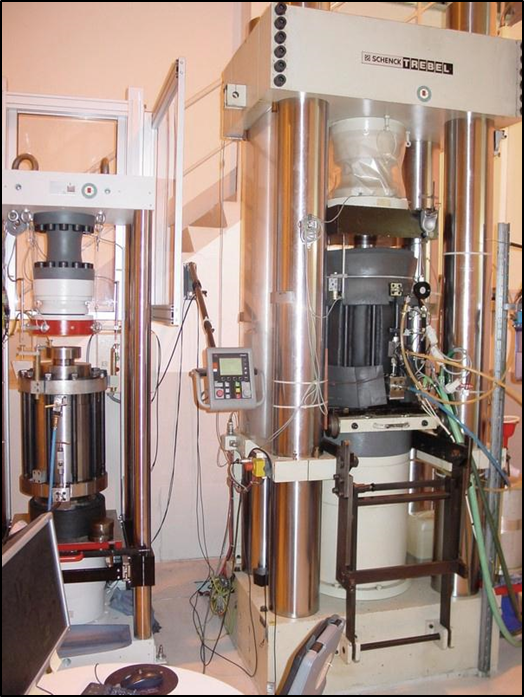
\includegraphics[width=0.5\textwidth]{./figures/ifg-lab-photo3.png}
\caption{The two available servo-controlled hydraulic testing machines (right: system RBA 2500 of SCHENK/TREBEL and left: D2000 of GGL TestSystems)}.
\label{fig:ifglabph2}
\end{figure}
